\documentclass{classrep}
\usepackage[utf8]{inputenc}
\usepackage{color}
\usepackage{enumitem}
\usepackage{graphicx}
\usepackage{amsmath}
\usepackage{float}
\usepackage{hyperref}

\studycycle{Informatyka, studia dzienne, I st.}
\coursesemester{VI}

\coursename{Komputerowe systemy rozpoznawania}
\courseyear{2019/2020}

\courseteacher{dr hab. inż. Adam Niewiadomski prof. uczelni}
\coursegroup{pon., 12:15}

\author{
\studentinfo{Mateusz Walczak}{216911} \and
\studentinfo{Konrad Kajszczak}{216790}
}

\title{Zadanie 2: Lingwistyczne podsumowania baz danych}
\svnurl{https://github.com/Walducha1908/KSR2}

\begin{document}
\maketitle

\section{Cel}
\textit{Praca w toku}


\section{Wprowadzenie}
\textit{Praca w toku}


\section{Opis implementacji}
\textit{Praca w toku}


\section{Materiały i metody}
Wybrana przez nas baza danych zawiera historyczne pomiary pogodowe z Holandii \cite{baza}. Dane zostały zgromadzone przez KNMI (\textit{Dutch weather institute} - Holenderski instytut pogodowy) na przestrzeni lat 1901-2018 i pochodziły z 50 różnych stacji pogowych znajdujących się na terenie całego kraju.\newline

Ze względu na fakt, iż oryginalna baza danych składa się z 804099 krotek, postanowiliśmy wybrać tylko niewielką część z dostępnych danych. Zdecydowaliśmy się na najnowsze dane pomiarowe - z lat 2016-2018. W ten sposób ograniczyliśmy liczbę wykorzystywanych krotek do 17000.\newline

\subsection{Wybór kolumn}
W celu analizy bazy danych i tworzenia jej lingwistycznych podsumowań wybraliśmy następujące 10 kolumn z danymi liczbowymi:

\begin{itemize}[label=$\bullet$\scshape\bfseries]
\item FG - średnia prędkość wiatru przez cały dzień [$0.1 \frac{m}{s}$].
\item FHX - najwyższa średnia prędkość wiatru w ciągu jednej godziny [$0.1 \frac{m}{s}$].
\item FHN - najniższa średnia prędkość wiatru w ciągu jednej godziny [$0.1 \frac{m}{s}$].
\item FXX - najszybszy podmuch wiatru w ciągu całego dnia [$0.1 \frac{m}{s}$].
\item TG - średnia dzienna temperatura [$0.1^{\circ} C$].
\item TN - minimalna dzienna temperatura [$0.1^{\circ} C$].
\item TX - maksymalna dzienna temperatura [$0.1^{\circ} C$].
\item T10N - minimalna dzienna temperatura na wysokości 10 cm od poziomu gruntu [$0.1^{\circ} C$].
\item Q - nasłonecznienie, energia słoneczna przypadająca na powierzchnię [$\frac{J}{cm^2}$].
\item RH - suma opadów atmosferycznych w ciągu całegi dnia [$0.1 mm$].\newline
\end{itemize}

Oprócz wyżej opisanych danych liczbowych, w naszej bazie znajdują się także dwie dodatkowe kolumny, służące do identyfikacji pomiaru:
\begin{itemize}[label=$\bullet$\scshape\bfseries]
\item STN - numer stacji badawczej wykonującej pomiar.
\item YYYYMMDD - data pomiaru w formacie opisanym przez nazwę kolumny.
\end{itemize}

\begin{figure}[H]
	\centering
	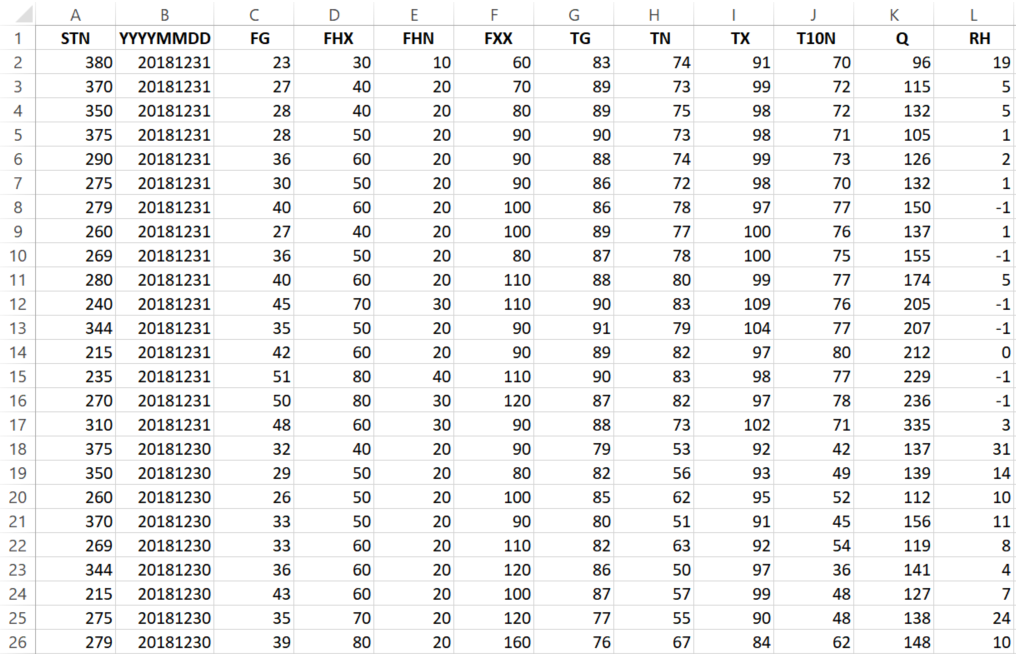
\includegraphics[width=1\textwidth]{Pictures/baza.png}
	\caption{Fragment widoku bazy w formacie $xlsx$}
\end{figure}






\subsection{Przykładowe zmienne lingwistyczne}
W tym rozdziale przedstawimy wzory i wykresy opisujące zaproponowane przez nas zmiennie lingwistyczne. We wszystkich przypadkach, wykorzystywanymi przez nas funkcjami przynależności są funkcje trapezoidalne.  \footnote{Wartości prezentowane w tabelach są tylko propozycjami. Autorzy sprawozdania zastrzegają sobie możliwość do ich późniejszej modyfikacji}.\newline

Ogólna postać funkcji trapezoidalnej, opisana jest wzorem:
\begin{equation}
{FG}_{GENTLE}(x)= \left\{ \begin{array}{ll}
\frac{x-a}{b-a} 	& \textrm{jeśli $a \leq x < b$} \\
1 			& \textrm{jeśli $b \leq x \leq c$} \\
\frac{d-x}{d-c} 	& \textrm{jeśli $c < x \leq d$} \\
0 			& \textrm{w przeciwnym wypadku.} \\
\end{array} \right.
\end{equation}

Aby nie duplikować treści wzorów, niepotrzebnie zwiększając w ten sposób objętość sprawozdania, zdecydowano się na zamieszczenie tabel z parametrami etykiet zmienny lingwistycznych, odnoszącymi się do powyższego wzoru.



\subsubsection{Kolumna FG}
Wykres opisujący zmienną lingwistyczną dla kolumny zawierającej wartości średniej prędkości wiatru przez cały dzień (FG), zamieszczono poniżej.
\begin{figure}[H]
	\centering
	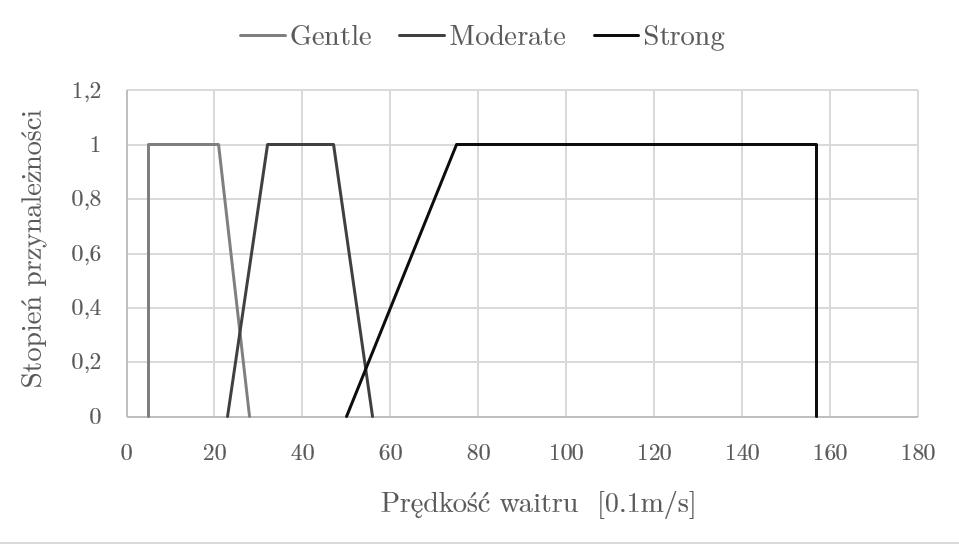
\includegraphics[width=0.99\textwidth]{Pictures/TermsCharts/FG.png}
	\caption{Wykres opisujący zmienną lingwistyczną dla kolumny FG.}
\end{figure}

\begin{table}[H]
	\centering
	\begin{tabular}{c c c c c} 
		\hline
		\textbf{Etykieta} & \textbf{a} & \textbf{b} & \textbf{c} & \textbf{d}\\ [0.5ex] 
		\hline
		\hline 
Gentle	 & 5 & 5 & 21 & 28 \\
Moderate & 23 & 32 & 47 & 56 \\
Strong	 & 50 & 75 & 157 & 157 \\
		\hline
	\end{tabular}
	\caption{Przyporządkowane parametry funkcji trapezoidalnej dla kolumny FG.}
\end{table}



\subsubsection{Kolumna TG}
W przypadku średniej dziennej temperatury (TG), zdecydowaliśmy się podzielić nasze rozważania ze względu na pory roku. Dlatego też przyjęliśmy trzy różne warianty zmiennej lingiwstycznej dla kolumny TG:

\begin{itemize}[label=$\bullet$\scshape\bfseries]
\item TGW - dla pomiarów uzyskanych podczas astronomicznej zimy (litera $W$ od $Winter$),
\item TGSA - dla pomiarów uzyskanych podczas astronomicznej wiosny lub jesieni ($S$ od $Spring$, $A$ od $Autumn$),
\item TGS -dla pomiarów uzyskanych podczas astronomicznego lata  (litera $S$ od $Summer$).\newline\newline
\end{itemize}

Rozpocznijmy od zmiennej lingwistycznej TGW.
\begin{figure}[H]
	\centering
	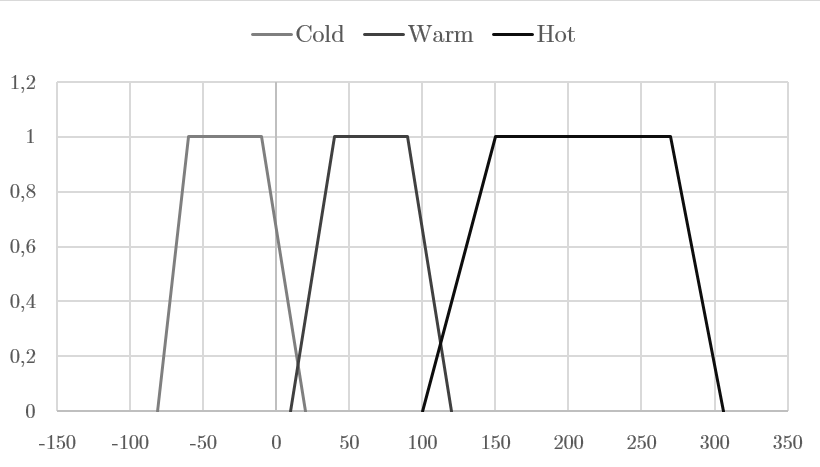
\includegraphics[width=0.99\textwidth]{Pictures/TermsCharts/TG_Z.png}
	\caption{Wykres opisujący zmienną lingwistyczną dla kolumny TG dla pomiarów wykonanych astronomiczną zimą.}
\end{figure}

\begin{table}[H]
	\centering
	\begin{tabular}{c c c c c} 
		\hline
		\textbf{Etykieta} & \textbf{a} & \textbf{b} & \textbf{c} & \textbf{d}\\ [0.5ex] 
		\hline
		\hline 
Cold	 &-81 & -81 & -10 & 20 \\
Warm & 10 & 40 & 90 & 120 \\
Hot	 & 100 & 150 & 306 & 306 \\
		\hline
	\end{tabular}
	\caption{Przyporządkowane parametry funkcji trapezoidalnej dla zmiennej TGW.}
\end{table}



Następną prezentowaną zmienną, będzie zmienna lingwistyczna TGSA.
\begin{figure}[H]
	\centering
	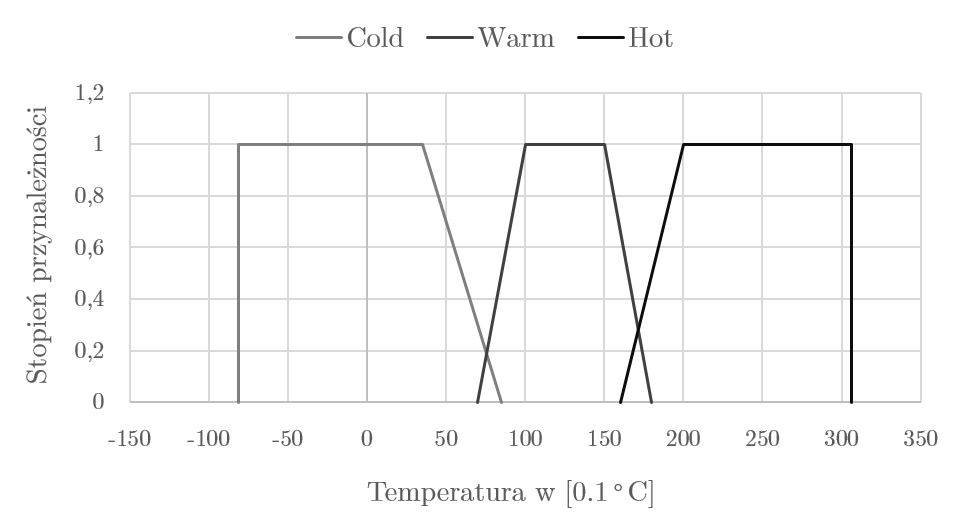
\includegraphics[width=0.99\textwidth]{Pictures/TermsCharts/TG_WJ.png}
	\caption{Wykres opisujący zmienną lingwistyczną dla kolumny TG dla pomiarów wykonanych astronomiczną wiosną i jesienią.}
\end{figure}

\begin{table}[H]
	\centering
	\begin{tabular}{c c c c c} 
		\hline
		\textbf{Etykieta} & \textbf{a} & \textbf{b} & \textbf{c} & \textbf{d}\\ [0.5ex] 
		\hline
		\hline 
Cold	 &-81 & -81 & 35 & 85 \\
Warm & 70 & 100 & 150 & 180 \\
Hot	 & 160 & 200 & 306 & 306 \\
		\hline
	\end{tabular}
	\caption{Przyporządkowane parametry funkcji trapezoidalnej dla zmiennej TGSA.}
\end{table}


Ostatnią zmienną dla kolumny TG będzie zmienna dotycząca pomiarów letnich - TGS.
\begin{figure}[H]
	\centering
	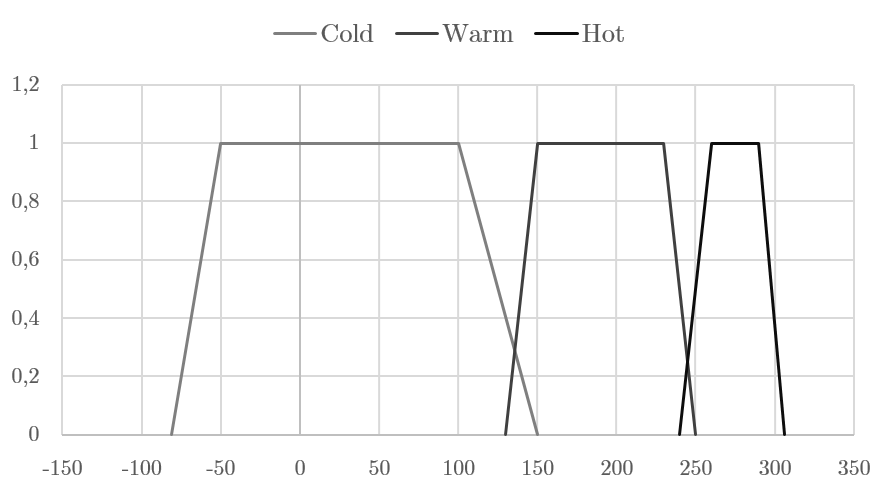
\includegraphics[width=0.99\textwidth]{Pictures/TermsCharts/TG_L.png}
	\caption{Wykres opisujący zmienną lingwistyczną dla kolumny TG dla pomiarów wykonanych astronomicznym latem.}
\end{figure}

\begin{table}[H]
	\centering
	\begin{tabular}{c c c c c} 
		\hline
		\textbf{Etykieta} & \textbf{a} & \textbf{b} & \textbf{c} & \textbf{d}\\ [0.5ex] 
		\hline
		\hline 
Cold	 &-81 & -81 & 100 & 150 \\
Warm & 130 & 150 & 230 & 250 \\
Hot	 & 240 & 260 & 306 & 306 \\
		\hline
	\end{tabular}
	\caption{Przyporządkowane parametry funkcji trapezoidalnej dla zmiennej TGS.}
\end{table}






\subsubsection{Kolumna Q}
Wykres opisujący zmienną lingwistyczną dla kolumny zawierającej wartości nasłonecznienia (Q), zamieszczono poniżej.
\begin{figure}[H]
	\centering
	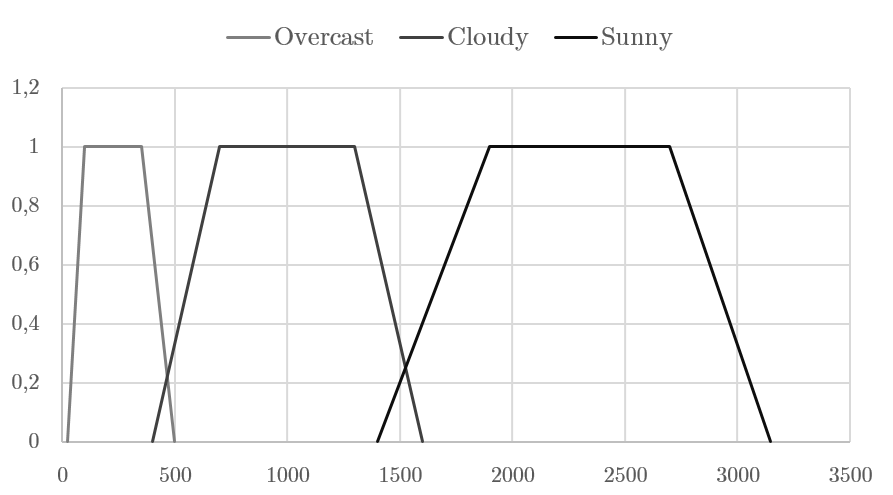
\includegraphics[width=0.99\textwidth]{Pictures/TermsCharts/Q.png}
	\caption{Wykres opisujący zmienną lingwistyczną dla kolumny Q}
\end{figure}

\begin{table}[H]
	\centering
	\begin{tabular}{c c c c c} 
		\hline
		\textbf{Etykieta} & \textbf{a} & \textbf{b} & \textbf{c} & \textbf{d}\\ [0.5ex] 
		\hline
		\hline 
Overcast	 & 24 & 24 & 350 & 500 \\
Cloudy & 400 & 700 & 1300 & 1600 \\
Sunny	 & 1400 & 1900 & 3145 & 3145 \\
		\hline
	\end{tabular}
	\caption{Przyporządkowane parametry funkcji trapezoidalnej dla kolumny Q.}
\end{table}




\section{Wyniki}
\textit{Praca w toku}


\section{Dyskusja}
\textit{Praca w toku}


\section{Wnioski}
\textit{Praca w toku}


\begin{thebibliography}{1}
\bibitem{baza} 
Baza danych - 
\href{https://www.kaggle.com/sinaasappel/historical-weather-in-the-netherlands-19012018}{\textit{"Historical weather in the Netherlands 1901-2018"}}
\end{thebibliography}
\end{document}
